%! TEX root = main.tex

\graphicspath{{00_Images/12_chapter/}}

\chapter{Condenser and MEMS Microphones}
\label{ch:condenser_mems}

\section{The Condenser Principle}
\label{sc:121}

The condenser (or capacitor) microphone is the most widely used transducer in precision measurement and studio recording, offering the best combination of flat frequency response, low self-noise, and extended bandwidth among all microphone types.
Its operating principle was first formalized by E.C. Wente in 1917 in a paper published in Physical Review, produced at the Research Laboratory of the American Telephone \& Telegraph Co. and Western Electric Co., where the device was described as a condenser transmitter for the absolute measurement of sound intensity.
The word transmitter reflected the primary application of the day: converting acoustic signals to electrical form for long-distance telephone transmission.
The theoretical treatment that followed in L.Beranek's textbook on acoustics established the electrostatic microphone as the standard for precision measurement, a role it retains today.

\subsection{Capacitance and Constant-Charge Operation}

A condenser microphone consists of a thin, tensioned diaphragm placed in close proximity to a rigid backplate, forming a parallel-plate capacitor whose capacitance varies with the instantaneous separation between the two electrodes.
The equilibrium capacitance is:
\[
C_0 = \varepsilon_0 \frac{A}{d_0}
\]
where \( A \) is the effective diaphragm area, \( d_0 \) is the rest-position gap, and \( \varepsilon_0 \) is the permittivity of free space.
The charge and voltage across the capacitor are linked by:
\[
Q = CV
\]
so that at equilibrium the bias voltage is \( V_B = Q_B / C_0 \), where \( Q_B \) is the bias charge placed on the capacitor.
The fundamental transduction principle is to maintain \( Q_B \) constant while the gap varies under acoustic pressure, so that any change in capacitance produces a proportional change in terminal voltage.
Holding the charge constant requires that the bias circuit present an extremely high impedance to the capsule: any charge leakage through a finite resistance \( R \) would discharge the capacitor on the time scale \( \tau = RC_0 \), and if \( \tau \) is comparable to the period of the audio signal, the low-frequency response degrades.

\subsection{Derivation of the Output Voltage}

When acoustic pressure \( p \) displaces the diaphragm by \( \Delta d \) toward the backplate, the new capacitance is:
\[
C = \varepsilon_0 \frac{A}{d_0 - \Delta d} \approx C_0 \left(1 + \frac{\Delta d}{d_0}\right)
\]
where the approximation holds for the small-signal regime \( |\Delta d| \ll d_0 \).
The incremental change in capacitance is therefore:
\[
\Delta C = C - C_0 \approx C_0 \frac{\Delta d}{d_0}
\]
With the charge held fixed at \( Q_B \), the new terminal voltage is \( V_B + V_S = Q_B/(C_0 + \Delta C) \), giving a signal voltage:
\begin{align*}
V_S &= Q_B\!\left(\frac{1}{C_0 + \Delta C} - \frac{1}{C_0}\right)
= Q_B \frac{-\Delta C}{C_0(C_0 + \Delta C)} \\
&\approx -\frac{Q_B}{C_0}\frac{\Delta C}{C_0}
= -V_B \frac{\Delta C}{C_0}
\end{align*}
Substituting the expression for \( \Delta C \):
\[
V_S \approx -V_B \frac{\Delta C}{C_0} \approx V_B \frac{\Delta d}{d_0}
\]
A displacement toward the backplate (compression) increases the capacitance and decreases the terminal voltage, consistent with the negative sign before \( \Delta C / C_0 \).
The signal voltage is therefore directly proportional to the diaphragm displacement, as illustrated in figure \ref{fig:condenserCrossSection}.

\begin{figure}[!htb]
    \centering
    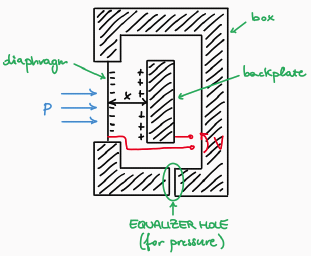
\includegraphics[width=0.55\textwidth]{condenser_mic.png}
    \caption{Simplified cross-section of a condenser microphone capsule: the tensioned diaphragm and the rigid backplate form a variable capacitor, and the vent hole provides static pressure equalization at the rear of the diaphragm}
    \label{fig:condenserCrossSection}
\end{figure}

\subsection{Stiffness-Controlled Regime and Sensitivity}

At audio frequencies well below the diaphragm resonance, the displacement is governed by the elastic restoring force of the diaphragm rather than by its inertia, so the system operates in the stiffness-controlled regime.
The displacement is proportional to the applied force:
\[
\Delta d = C_{MS}F = C_{MS}pS_D
\]
where \( C_{MS} \) is the mechanical compliance of the diaphragm.
Substituting into the signal voltage expression and using \( V_B/d_0 = Q_B/(\varepsilon_0A) \):
\[
V_S = \frac{Q_B}{\varepsilon_0A}C_{MS}pS_D = \frac{Q_B}{\varepsilon_0}C_{MS}p
\]
since \( A \equiv S_D \).
The open-circuit sensitivity of the condenser microphone is therefore:
\[
\mathcal{S} = \frac{V_S}{p} = \frac{Q_B}{\varepsilon_0}C_{MS}
\]
The sensitivity increases with the bias charge and with the mechanical compliance of the diaphragm.
A softer diaphragm produces a larger displacement for a given pressure, yielding higher sensitivity; conversely, a stiffer diaphragm raises the resonance frequency and extends the flat response region.
This stiffness-controlled operation contrasts with the electrodynamic loudspeaker, which operates in a mass-controlled regime above its mechanical resonance.

\begin{figure}[!htb]
    \centering
    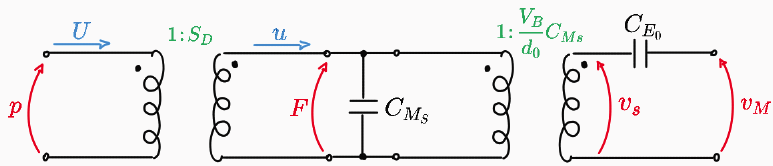
\includegraphics[width=0.70\textwidth]{condenser_mic_equiv_circuit.png}
    \caption{Equivalent electromechanical circuit of the condenser capsule: acoustic pressure \( p \) produces the force \( F = pS_D \) acting on the diaphragm compliance \( C_{MS} \), and the resulting displacement modulates the electrical capacitance \( C_{E0} \) to produce the output signal voltage}
\end{figure}

\subsection{Electret Microphones}

A standard condenser microphone requires an external bias voltage, typically \SI{48}{\volt} of phantom power, to establish the charge \( Q_B \) on the capsule.
An electret microphone eliminates this external requirement by permanently polarizing the backplate or the diaphragm with a dielectric material that retains a built-in electrostatic charge.
The backplate is coated with a fluoropolymer film, typically fluorinated ethylene propylene (FEP): during manufacture the material is heated above its glass transition temperature, subjected to a strong electric field, and cooled with the field applied, freezing the aligned molecular dipoles in place and creating a permanently embedded surface charge equivalent to the external bias.

\begin{figure}[!htb]
    \centering
    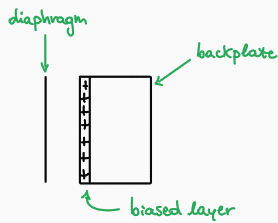
\includegraphics[width=0.35\textwidth]{electret_mic_structure.png}
    \caption{Cross-section of an electret capsule: the permanently polarized dielectric layer on the backplate supplies the bias charge \( Q_B \) without requiring an external polarization supply}
\end{figure}

The sensitivity expression \( \mathcal{S} = Q_BC_{MS}/\varepsilon_0 \) applies identically to electret and externally polarized designs; the only distinction is the source of \( Q_B \).
An internal impedance converter is still required to extract the signal from the high-impedance capsule, and it is powered via phantom power or a small internal battery.
Modern electret capsules achieve performance virtually indistinguishable from externally polarized types and represent the large majority of condenser microphones produced, including essentially all consumer, communication, and MEMS devices.

\section{Internal Electronics and Phantom Power}
\label{sc:122}

The condenser capsule presents a source impedance that is nearly that of a pure capacitance of a few picofarads, which at audio frequencies corresponds to a source impedance on the order of hundreds of megaohms.
This extremely high impedance makes the signal vulnerable to loading by any parasitic capacitance in the signal path before the first amplifying stage.

\subsection{The Cable Capacitance Problem}

When the microphone capsule is connected to a cable without an internal buffer, the capsule capacitance \( C_{E0} \) forms a capacitive voltage divider with the sum of the cable capacitance and the preamplifier input capacitance.
Typical values for a professional installation are:
\[
C_{E0} \approx \SI{10}{\pico\farad}, \qquad
C_{\mathrm{IN}} \approx \SI{10}{\pico\farad}, \qquad
C_{\mathrm{cable}} \approx \SI{100}{\pico\farad\per\meter}
\]
For a cable of length \( l = \SI{1}{\meter} \), the fraction of the signal recovered at the preamplifier input is:
\[
\frac{v_{\mathrm{IN}}}{v_s} = \frac{C_{E0}}{C_{E0} + C_{\mathrm{cable}}l + C_{\mathrm{IN}}}
= \frac{10}{10 + 100 + 10}
\approx \frac{1}{12}
< 10\%
\]
More than \SI{90}{\percent} of the signal is dissipated in the capacitive divider before it reaches the preamplifier, an unacceptable loss for any precision audio system.

\begin{figure}[!htb]
    \centering
    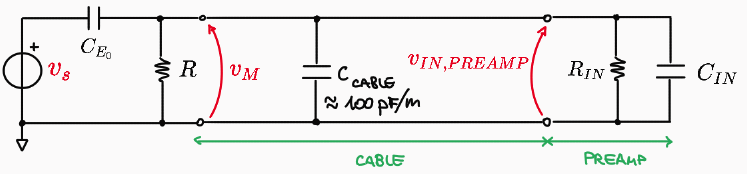
\includegraphics[width=0.60\textwidth]{microphone_cable_effect.png}
    \caption{Capacitive loading of the unshielded condenser capsule: the capsule capacitance \( C_{E0} \), the cable capacitance \( C_{\mathrm{cable}} \), and the preamplifier input capacitance \( C_{\mathrm{IN}} \) form a voltage divider; without an internal buffer, a \SI{1}{\meter} cable recovers less than 10\% of the signal}
\end{figure}

The solution is to integrate an impedance converter, typically a JFET source follower, directly inside the microphone body and as close to the capsule as physically possible.
The JFET gate presents an input impedance in excess of \SI{1}{\giga\ohm} to the capsule, and the source presents a low output impedance of a few hundred ohms to the cable.
With the buffer in place, the cable capacitance loads the JFET output rather than dividing the capsule voltage directly, and the signal attenuation becomes negligible.
A large bias resistor \( R_B \), typically several hundred megaohms, establishes the DC gate potential and forms a high-pass RC network with the capsule capacitance; the cutoff frequency is:
\[
f_L = \frac{1}{2\pi R_BC_{E0}}
\]
For \( C_{E0} = \SI{10}{\pico\farad} \) and the requirement \( f_L \leq \SI{20}{\hertz} \), the minimum bias resistance is:
\[
R_B \geq \frac{1}{2\pi \cdot \SI{20}{\hertz} \cdot \SI{10}{\pico\farad}} \approx \SI{800}{\mega\ohm}
\]

\begin{figure}[!htb]
    \centering
    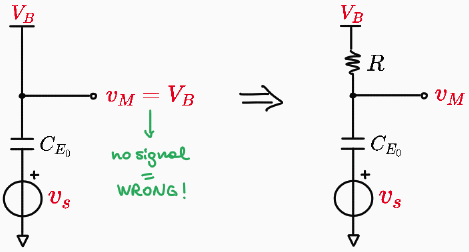
\includegraphics[width=0.50\textwidth]{electret_mic_bias_circuit.png}
    \caption{Bias and coupling circuit for signal extraction from a condenser capsule: the large resistor \( R_B \) establishes the JFET gate potential while the coupling capacitor isolates the AC signal; the RC network functions as a high-pass filter with cutoff \( f_L = 1/(2\pi R_B C_{E0}) \)}
\end{figure}

\subsection{Phantom Power}

The internal impedance converter and any subsequent preamplifier stages require an operating voltage.
Rather than a separate power cable or internal battery, professional condenser microphones use phantom power: the operating voltage is delivered over the same balanced cable that carries the audio signal, completely transparent to the audio system.
The standard phantom supply voltage is \( V_{\mathrm{BIAS}} = \SI{48}{\volt} \) (IEC 61938), though voltages between \SI{11}{\volt} and \SI{52}{\volt} are found in practice depending on the application.
The supply voltage is applied to the center tap of the output transformer inside the microphone, or equivalently through two equal resistors connected to pins 2 and 3 of the XLR connector in a transformerless design.
Both signal conductors carry the same DC potential \( V_{\mathrm{BIAS}} \) with respect to the shield, and the total current \( I \) consumed by the preamplifier divides equally as \( I/2 \) in each conductor.
At the preamplifier end, the differential input amplifies only the voltage difference between the two conductors: since both carry the same DC level, the phantom supply produces no net differential signal, and it does not appear at the audio output.

\begin{figure}[!htb]
    \centering
    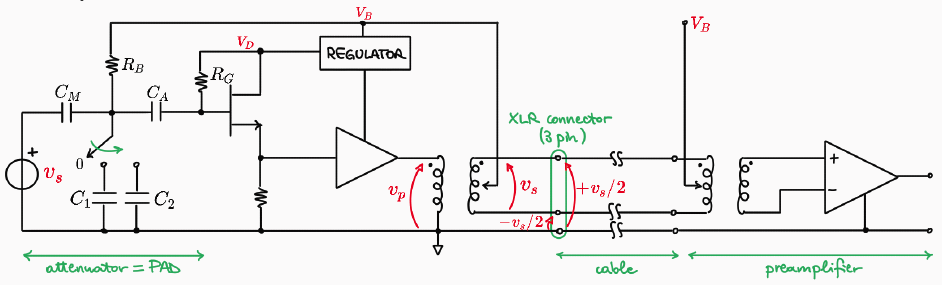
\includegraphics[width=0.85\textwidth]{phantom_power.png}
    \caption{Phantom power circuit architecture: the bias voltage \( V_{\mathrm{BIAS}} \) is fed symmetrically to both signal conductors through equal resistors; the stationary current \( I \) splits as \( I/2 \) in each leg, supplying power to the internal preamplifier without appearing as a differential audio signal}
\end{figure}

\paragraph{Common-mode rejection of supply disturbances} Consider a disturbance current \( i \) superimposed on the nominal supply current, arising for instance from power-supply ripple or electromagnetic pickup on the cable.
Because the phantom topology is symmetric, the disturbance distributes equally as \( i/2 \) in each conductor, producing an identical voltage perturbation \( v/2 \) on both lines.
The differential voltage presented to the preamplifier input is:
\[
v_{\mathrm{diff}}
= \left(V_{\mathrm{BIAS}} + \frac{v}{2}\right)
- \left(V_{\mathrm{BIAS}} + \frac{v}{2}\right) = 0
\]
The disturbance is a pure common-mode signal and is rejected by the differential amplifier stage.
The common-mode rejection ratio (CMRR) of professional microphone preamplifiers is typically \SI{60}{\decibel} or higher across the audio band, attenuating the residual interference by a factor of at least 1000.
This is the fundamental advantage of the balanced differential connection used in all professional audio installations: any electromagnetic interference induced equally on both conductors cancels at the differential input, while the desired audio signal, which is transmitted as a differential voltage \( +v_s/2 \) on one conductor and \( -v_s/2 \) on the other, is unaffected.

\begin{figure}[!htb]
    \centering
    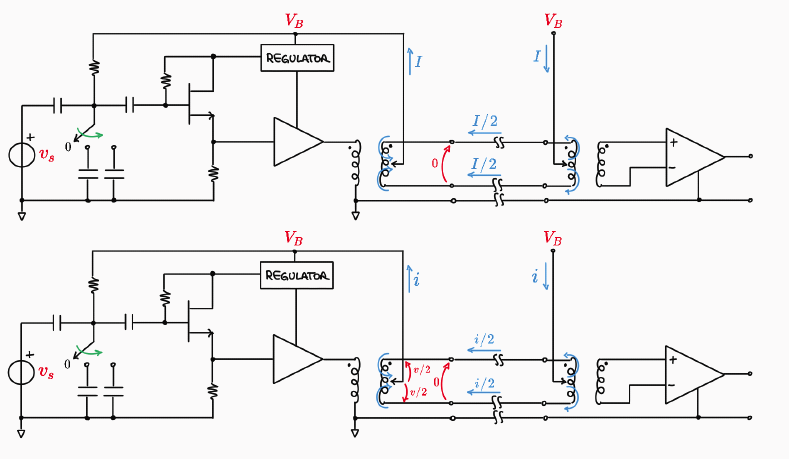
\includegraphics[width=0.85\textwidth]{phantom_power_2.png}
    \caption{Common-mode rejection in the phantom power line: the stationary supply current \( I \) and a superimposed disturbance \( i \) both distribute symmetrically as \( (I+i)/2 \) on each conductor; the disturbance voltages \( v/2 \) appear identically on both lines and cancel at the differential preamplifier input, leaving the audio signal intact}
\end{figure}

\subsection{Complete Internal Electronics Chain}

A representative internal electronics chain, exemplified by designs such as the Shure SM81 or the AKG C-460B, includes the following functional stages in cascade: a capacitive attenuator pad for operation at high sound pressure levels up to \SI{145}{\decibel} SPL; a JFET source follower as the primary impedance converter; a passive high-pass RC filter network providing switchable low-frequency roll-off (flat, \SI{-6}{\decibel\per\octave} at \SI{100}{\hertz}, or \SI{-18}{\decibel\per\octave} at \SI{80}{\hertz}); a BJT buffer for additional current drive capacity; and an output transformer that converts the single-ended capsule signal to a balanced differential output while injecting the phantom supply voltage at its center tap.
In transformerless designs, the balanced output is produced by a symmetric active output stage followed by two DC-blocking capacitors, and the phantom voltage is injected through two matched resistors directly at the connector.
Every component in the high-impedance node preceding the JFET gate must be designed for minimum thermal noise, since even a single resistor at this node can dominate the noise floor of the entire microphone.


\section{MEMS Microphones}
\label{sc:123}

Micro-Electro-Mechanical Systems (MEMS) microphones represent the most recent evolution of the condenser transduction principle and now constitute the dominant microphone technology by units produced worldwide.
By applying the photolithographic fabrication techniques of integrated circuit manufacturing to acoustic transducers, MEMS technology enables the production of complete microphone capsules at the scale and per-unit cost of passive electronic components, with dimensional control at the sub-micrometer level.

\subsection{The MEMS Concept}

MEMS is the integration of mechanical elements, sensors, actuators, and electronics on a common silicon substrate through microfabrication technology.
The electronic components are fabricated using standard IC process sequences such as CMOS, Bipolar, or BiCMOS, while the micromechanical structures are produced by compatible micromachining processes that selectively etch away regions of the silicon wafer or deposit new structural layers to form movable mechanical elements.
In the context of microphones, the mechanical element is a thin silicon diaphragm suspended above a rigid perforated backplate, reproducing the diaphragm-and-backplate geometry of a conventional condenser capsule at a scale of hundreds of micrometers.

\subsection{Silicon Microfabrication Technology}

The starting material for all silicon microfabricated devices is a monocrystalline silicon wafer of electronic-grade purity.
Metallurgic-grade silicon, obtained by reducing silicon dioxide with carbon in an arc furnace:
\[
\mathrm{SiC(s)} + \mathrm{SiO_2(s)} \longrightarrow \mathrm{Si(s)} + \mathrm{SiO(g)} + \mathrm{CO(g)}
\]
achieves a purity of approximately 98\%, which is insufficient for electronic applications.
Further purification to electronic grade reduces the total impurity concentration (boron, copper, gold, iron, chromium, manganese, and others) to below \( 10^{13} \) atoms per \si{\centi\meter\cubed}, against a silicon atom concentration of \( 10^{22} \) atoms per \si{\centi\meter\cubed}, corresponding to a purity of \( 10^{-3} \) ppm, or 99.9999999\%.
Monocrystalline ingots are grown from this purified material by the Czochralski process: a small seed crystal is dipped into a quartz crucible containing molten silicon held at the silicon fusion temperature of \( \SI{1415}{\degreeCelsius} \), then slowly withdrawn and rotated, pulling a single-crystal ingot with a diameter between \SI{4}{\inch} and \SI{12}{\inch}.
The ingot is sliced into wafers of thickness between \SI{300}{\micro\meter} and \SI{500}{\micro\meter}, which are then lapped and polished to a surface flatness variation below \SI{1}{\micro\meter}, providing the planar substrate required for photolithographic processing.
The primary microfabrication steps applied to each wafer are as follows.

\paragraph{Thermal oxidation} Heating the wafer in an oxidizing atmosphere grows a conformal layer of silicon dioxide (\(\mathrm{SiO_2}\)) by consuming the silicon surface; this oxide serves as an electrical insulator, a diffusion mask for subsequent doping steps, and a sacrificial layer that can be selectively removed later to release mechanical structures.

\paragraph{Photolithography} A photosensitive polymer (photoresist) is spin-coated onto the wafer, exposed through a reticle carrying the desired pattern using ultraviolet light, and developed to reveal the exposed areas; the resulting patterned mask protects selected regions during etching, enabling the definition of features with lateral dimensions below one micrometer.

\paragraph{Etching} Both wet chemical etching using solutions such as KOH for anisotropic silicon removal and HF for silicon dioxide, and dry plasma etching using reactive ion processes, are employed to sculpt the three-dimensional microstructure; in MEMS acoustic devices, a deep anisotropic etch through the full wafer thickness forms the back cavity that acoustically loads the diaphragm and defines the backvolume of the capsule.
After all structural and electrical layers have been deposited and patterned, a final release etch removes the sacrificial oxide beneath the diaphragm, freeing it from the substrate and leaving it suspended above the backplate by an air gap of precisely controlled thickness.

\subsection{MEMS Microphone Structure and Fabrication Routes}

A MEMS microphone capsule reproduces, at microscale, the diaphragm-and-backplate geometry of a conventional condenser capsule.
The diaphragm is a thin circular membrane of LPCVD (low-pressure chemical vapor deposited) silicon nitride or polysilicon, typically \SI{0.5}{\micro\meter} to \SI{2}{\micro\meter} thick, deposited under controlled conditions to achieve a prescribed residual tensile stress that governs its compliance and resonance frequency.
The backplate is a rigid electrode perforated with acoustic holes that allow air to flow freely through the gap, preventing the sealed air volume from acting as an additional stiffness in series with the diaphragm suspension.
Two main fabrication routes are used in practice.
In the two-wafer bonding process, the diaphragm and backplate are fabricated independently on two separate wafers: the diaphragm wafer undergoes oxide formation, silicon nitride deposition, and electrode patterning, while the backplate wafer is etched to define the acoustic holes and stiffening geometry; the two wafers are then bonded face-to-face by gold-gold thermocompression bonding, and the bonding pad height defines the air gap with sub-micrometer accuracy.
In the single-wafer surface micromachining process, a sacrificial oxide layer deposited at the start of the process defines the future gap thickness; polysilicon or silicon nitride is deposited on top to form the diaphragm; a final vapor-HF or wet-HF etch removes the sacrificial layer through the acoustic holes in the backplate, releasing the diaphragm on the same substrate without wafer bonding.

\subsection{Sensitivity and the Role of the Air Gap}

The key performance advantage of MEMS microphones originates directly from the small air gap dimension made possible by photolithographic processing.
The electrostatic pressure acting on the diaphragm per unit area, derived from the energy stored in the electric field, is:
\[
P_{\mathrm{el}} = \frac{\varepsilon_0V_B^2}{2d^2} \propto \frac{1}{d^2}
\]
Reducing the gap by a factor of ten at the same bias voltage increases the electrostatic force by a factor of one hundred.
The electric field \( \mathcal{E} = V_B/d \) scales inversely with gap, and the charge-to-voltage conversion efficiency \( V_S/\Delta d = V_B/d \) also scales inversely with gap, so a ten-fold reduction in gap yields a ten-fold improvement in sensitivity for the same diaphragm displacement.
In a conventional condenser capsule, the gap between diaphragm and backplate is typically on the order of \SI{20}{\micro\meter} to \SI{50}{\micro\meter}, limited by mechanical tolerances in the hand-assembly process.
In a MEMS device, the gap is defined by a deposited sacrificial oxide layer with a thickness of \SI{1}{\micro\meter} to \SI{4}{\micro\meter}, controlled to sub-micrometer accuracy by the deposition recipe.
This is the fundamental reason why MEMS microphones achieve sensitivity values comparable to much larger conventional capsules despite their millimeter-scale diaphragm area: the sub-micrometer gap generates an intense electric field from a modest bias voltage, compensating for the reduced electrode area.

\subsection{Commercial MEMS Microphones}

Commercial MEMS microphones are available in two output formats distinguished by the level of signal processing performed on-chip.
Analog MEMS microphones produce a continuous voltage output proportional to acoustic pressure; they include an on-chip JFET or CMOS impedance converter but no analog-to-digital conversion, and they interface to standard audio signal chains with supply voltages between \SI{1.5}{\volt} and \SI{5.5}{\volt} and current consumptions below \SI{250}{\micro\ampere}.
Digital MEMS microphones integrate a sigma-delta modulator alongside the MEMS capsule on the same die, producing a single-bit Pulse Density Modulation (PDM) bitstream at a clock frequency between \SI{1}{\mega\hertz} and \SI{4}{\mega\hertz}; this bitstream is decoded by an audio codec, DSP, or microcontroller, eliminating all analog conditioning in the downstream system and providing inherent immunity to electromagnetic interference on the signal lines.
The key practical advantages of MEMS microphones over conventional condenser capsules include their compact package size, with footprints on the order of \( 3\mathrm{mm} \times 4\mathrm{mm} \times 1\mathrm{mm} \); compatibility with automated surface-mount reflow soldering at temperatures up to \SI{260}{\degreeCelsius}, which eliminates hand-assembly; high resistance to mechanical shock; and exceptional unit-to-unit matching.
Because thousands of capsules are fabricated simultaneously on a single wafer under identical photolithographic conditions, matched pairs selected from the same batch exhibit sensitivity differences below \SI{1}{\decibel}, making MEMS microphones the enabling technology for stereo arrays, beamforming systems, and differential noise-cancellation configurations in smartphones, laptops, hearing aids, wearable devices, and industrial IoT sensors.
